\documentclass[11pt]{article}
\usepackage{fancyhdr}
\pagestyle{fancy}
\newcommand\course{MATH 423}
\newcommand\hwnumber{3}
\newcommand\duedate{October 31, 2019}

\lhead{Oliver Tonnesen\\V00885732}
\chead{\textbf{\Large Project \hwnumber}}
\rhead{\course\\\duedate}


\usepackage{cite}
\usepackage{url}


\usepackage{tikz}
\newcount\mycount


\usepackage{float}
\usepackage{subcaption}


\usepackage{amsmath,amsfonts,amsthm}


\begin{document}
\section{Definition and characterizations}

\subsection{Definition of a line graph}

A line graph of a simple graph $G$, $L(G)$, is the graph obtained by taking $E(G)$ to be its vertex set, and connecting two vertices with an edge if the corresponding edges in $G$ share a common vertex.

Some definitions we use throughout this survey, assume $H$ is a suspected line graph and $G$ is its root graph if it exists:
\newline
\underline{\textbf{$g$-clique}}: If $g\in G$, a $g$-clique in $H$ is a clique in $H$, corresponding to the star graph centred at $g$ in $G$.
\newline
\underline{\textbf{Half-named}}: A vertex in $H$ is "half-named" when it corresponds to an edge of $G$, one of whose vertices belongs to a fully
discovered $g$-clique in $H$.
\newline
\underline{\textbf{Fully named}}: A vertex in $H$ is "fully named" when it corresponds to an edge of $G$, both of whose vertices belong to a fully discovered $g$-clique in $H$.
\newline
\underline{\textbf{Even triangle}}: A triangle such that every vertex in the graph is adjacent to exactly two or zero vertices in the triangle.
\newline
\underline{\textbf{Odd triangle}}: A triangle such that every vertex in the graph is adjacent to exactly one or three vertices in the triangle.
\newline
\underline{\textbf{Cross vertex}}: Given two vertices in $H$ $x-y$ and $y-z$, a cross vertex is one of the form the name $x-z$.


\subsection{Examples}

\begin{figure}[H]
\centering
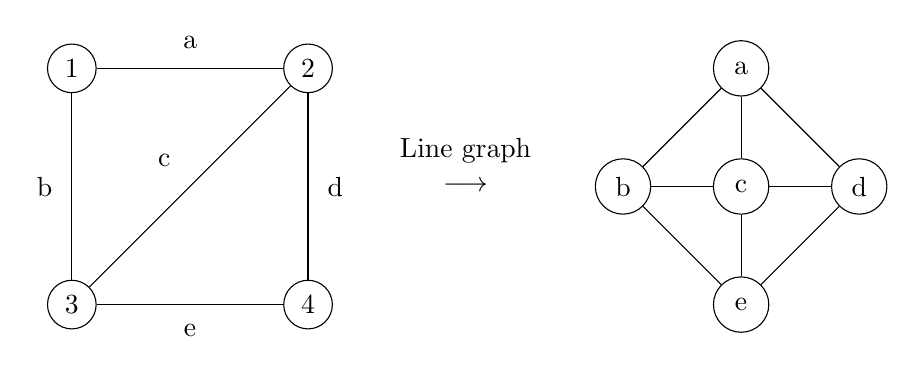
\begin{tikzpicture}[black/.style={circle,draw,fill=black,inner sep=0pt, minimum width=4pt}]
\node[circle,draw] at (0,3) (1) {1};
\node[circle,draw] at (3,3) (2) {2};
\node[circle,draw] at (0,0) (3) {3};
\node[circle,draw] at (3,0) (4) {4};

\draw (1) -- (2) node [midway,label=above:{a}] {};
\draw (1) -- (3) node [midway,label=left:{b}] {};
\draw (2) -- (3) node [midway,label=above left:{c}] {};
\draw (2) -- (4) node [midway,label=right:{d}] {};
\draw (3) -- (4) node [midway,label=below:{e}] {};


\draw node at (5, 1.5) {$\longrightarrow$};
\draw[above,yshift=5] node at (5,1.5) {Line graph};


\node[circle,draw,minimum width=20pt] at (8.5,3) (a) {a};
\node[circle,draw,minimum width=20pt] at (7,1.5) (b) {b};
\node[circle,draw,minimum width=20pt] at (8.5,1.5) (c) {c};
\node[circle,draw,minimum width=20pt] at (10,1.5) (d) {d};
\node[circle,draw,minimum width=20pt] at (8.5,0) (e) {e};

\draw (a) -- (b);
\draw (a) -- (c);
\draw (a) -- (d);
\draw (b) -- (c);
\draw (b) -- (e);
\draw (c) -- (d);
\draw (c) -- (e);
\draw (d) -- (e);
\end{tikzpicture}

\end{figure}
\begin{figure}[H]
\centering
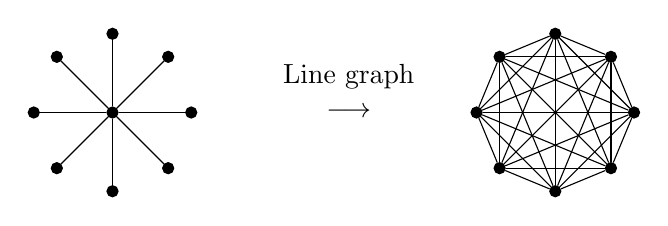
\begin{tikzpicture}[black/.style={circle,draw,fill=black,inner sep=0pt,minimum width=4pt}]
\node[black] at (0,0) (0) {};
\foreach \number in {1,...,8}
{
	\mycount=\number
	\advance\mycount by -1
	\multiply\mycount by 45
	\advance\mycount by 0
	\node[black] (\number) at (\the\mycount:1cm) {};
	\draw (0) -- (\number);
}


\draw node at (3, 0) {$\longrightarrow$};
\draw[above,yshift=5] node at (3,0) {Line graph};


\foreach \number in {1,...,8}
{
	\mycount=\number
	\advance\mycount by -1
	\multiply\mycount by 45
	\advance\mycount by 0
	\node[black,xshift=160] (\number) at (\the\mycount:1cm) {};
}
\foreach \x in {1,...,8}
	\foreach \y in {\x,...,8}
		\draw (\x) -- (\y);


\end{tikzpicture}

\end{figure}


\subsection{Characterizations of line graphs by forbidden structures and by forbidden subgraphs}

A graph is the line graph of some simple graph if and only if it contains none of these nine graphs as induced subgraphs \cite{vanRooij}:

\begin{figure}[H]
\centering
	\begin{minipage}{.3\textwidth}
		\centering
		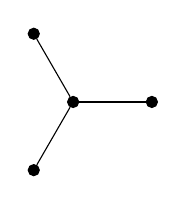
\begin{tikzpicture}[black/.style={circle,draw,fill=black,inner sep=0pt, minimum width=4pt}]
\node[black] at (0,0) (0) {};
\foreach \number in {1,...,3}
{
	\mycount=\number
	\advance\mycount by -1
	\multiply\mycount by 120
	\advance\mycount by 0
	\node[black] (\number) at (\the\mycount:1cm) {};
	\draw (0) -- (\number);
}
\end{tikzpicture}

	\end{minipage}
	\begin{minipage}{.3\textwidth}
		\centering
		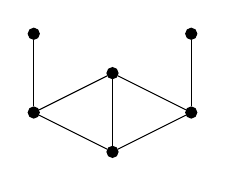
\begin{tikzpicture}[black/.style={circle,draw,fill=black,inner sep=0pt, minimum width=4pt}]
\node[black] at (1,0)	(0) {};
\node[black] at (0,0.5)	(1) {};
\node[black] at (2,0.5)	(2) {};
\node[black] at (1,1)	(3) {};
\node[black] at (0,1.5)	(4) {};
\node[black] at (2,1.5)	(5) {};

\draw (0) -- (1);
\draw (0) -- (2);
\draw (0) -- (3);
\draw (3) -- (1);
\draw (3) -- (2);
\draw (4) -- (1);
\draw (5) -- (2);
\end{tikzpicture}

	\end{minipage}
	\begin{minipage}{.3\textwidth}
		\centering
		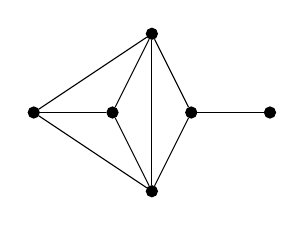
\begin{tikzpicture}[black/.style={circle,draw,fill=black,inner sep=0pt, minimum width=4pt}]
\node[black] at (0,0)	(0) {};
\node[black] at (1,0)	(1) {};
\node[black] at (1.5,1)	(2) {};
\node[black] at (1.5,-1)(3) {};
\node[black] at (2,0)	(4) {};
\node[black] at (3,0)	(5) {};

\draw (0) -- (1);
\draw (0) -- (2);
\draw (0) -- (3);
\draw (1) -- (2);
\draw (1) -- (3);
\draw (2) -- (3);
\draw (4) -- (2);
\draw (4) -- (3);
\draw (4) -- (5);
\end{tikzpicture}

	\end{minipage}
\end{figure}
\begin{figure}[H]
\centering
	\begin{minipage}{.3\textwidth}
		\centering
		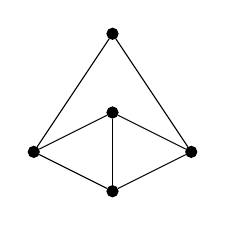
\begin{tikzpicture}[black/.style={circle,draw,fill=black,inner sep=0pt, minimum width=4pt}]
\node[black] at (1,0)	(0) {};
\node[black] at (0,0.5)	(1) {};
\node[black] at (2,0.5)	(2) {};
\node[black] at (1,1)	(3) {};
\node[black] at (1,2)	(4) {};

\draw (0) -- (1);
\draw (0) -- (2);
\draw (0) -- (3);
\draw (1) -- (3);
\draw (2) -- (3);
\draw (4) -- (1);
\draw (4) -- (2);
\end{tikzpicture}

	\end{minipage}
	\begin{minipage}{.3\textwidth}
		\centering
		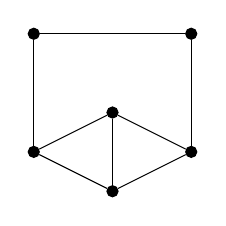
\begin{tikzpicture}[black/.style={circle,draw,fill=black,inner sep=0pt, minimum width=4pt}]
\node[black] at (1,0)	(0) {};
\node[black] at (0,0.5)	(1) {};
\node[black] at (2,0.5)	(2) {};
\node[black] at (1,1)	(3) {};
\node[black] at (0,2)	(4) {};
\node[black] at (2,2)	(5) {};

\draw (0) -- (1);
\draw (0) -- (2);
\draw (0) -- (3);
\draw (1) -- (3);
\draw (2) -- (3);
\draw (4) -- (1);
\draw (5) -- (2);
\draw (5) -- (4);
\end{tikzpicture}

	\end{minipage}
	\begin{minipage}{.3\textwidth}
		\centering
		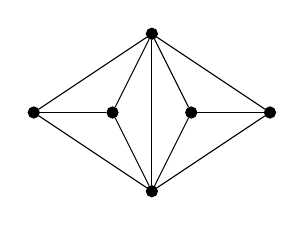
\begin{tikzpicture}[black/.style={circle,draw,fill=black,inner sep=0pt, minimum width=4pt}]
\node[black] at (0,0)	(0) {};
\node[black] at (1,0)	(1) {};
\node[black] at (1.5,1)	(2) {};
\node[black] at (1.5,-1)(3) {};
\node[black] at (2,0)	(4) {};
\node[black] at (3,0)	(5) {};

\draw (0) -- (1);
\draw (0) -- (2);
\draw (0) -- (3);
\draw (1) -- (2);
\draw (1) -- (3);
\draw (2) -- (3);
\draw (4) -- (2);
\draw (4) -- (3);
\draw (4) -- (5);
\draw (5) -- (2);
\draw (5) -- (3);
\end{tikzpicture}

	\end{minipage}
\end{figure}
\begin{figure}[H]
\centering
	\begin{minipage}{.3\textwidth}
		\centering
		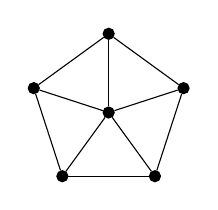
\begin{tikzpicture}[black/.style={circle,draw,fill=black,inner sep=0pt, minimum width=4pt}]
\node[black] at (0,0) (0) {};
\foreach \x in {1,...,5}
{
	\mycount=\x
	\advance\mycount by -1
	\multiply\mycount by 72
	\advance\mycount by 18
	\node[black] (\x) at (\the\mycount:1cm) {};
	\draw (0) -- (\x);
}
\foreach \x in {1,...,4}
{
	\mycount=\x
	\advance\mycount by 1
	\draw (\x) -- (\the\mycount);
}
\draw (1) -- (5);
\end{tikzpicture}

	\end{minipage}
	\begin{minipage}{.3\textwidth}
		\centering
		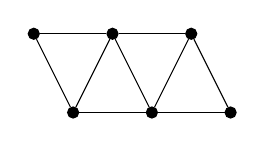
\begin{tikzpicture}[black/.style={circle,draw,fill=black,inner sep=0pt, minimum width=4pt}]
\foreach \x in {0,...,2}
{
	\node[black] at (\x, 1) (a\x) {};
	\node[black] at (\x+0.5, 0) (b\x) {};
	\draw (a\x) -- (b\x);
}
\foreach \x/\y in {0/1,1/2}
{
	\draw (a\x) -- (a\y);
	\draw (b\x) -- (b\y);
	\draw (b\x) -- (a\y);
}
\end{tikzpicture}

	\end{minipage}
	\begin{minipage}{.3\textwidth}
		\centering
		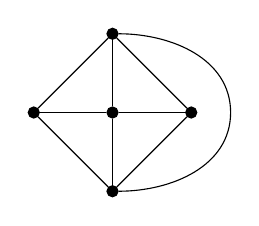
\begin{tikzpicture}[black/.style={circle,draw,fill=black,inner sep=0pt, minimum width=4pt}]
\node[black] at (0,0) (0) {};
\foreach \x in {1,...,4}
{
	\mycount=\x
	\advance\mycount by -1
	\multiply\mycount by 90
	\advance\mycount by 0
	\node[black] (\x) at (\the\mycount:1cm) {};
	\draw (0) -- (\x);
}
\foreach \x in {1,...,3}
{
	\mycount=\x
	\advance\mycount by 1
	\draw (\x) -- (\the\mycount);
}
\draw (1) -- (4);
\draw (2) to[out=0,in=90] (1.5,0) to[out=-90,in=0]  (4);
\end{tikzpicture}

	\end{minipage}
\end{figure}

Another characterization \cite{vanRooij}: A graph is a line graph of some simple graph if and only if it is claw-free and no induced diamond subgraph of $G$ has two odd triangles.


\section{Recognition}

\subsection{Lehot algorithm for constructing the root graph of a graph if it exists}

We're given a graph $G=(V(G),E(G)$. The algorithm described in \cite{Lehot} has 9 steps:
\newline
\newline
\noindent
\underline{Step 1}:
Select two adjacent vertices in $V(G)$, and name them $1-2$ and $2-3$.
Call these vertices the "basic vertices."
\newline
\newline
\noindent
\underline{Step 2}:
Find all vertices adjacent to both basic vertices.
If there are at least three such vertices, go to step 5.
If there are none, go to step 6.
If there is one, continue to step 3.
If there are two, go to step 4.
\newline
\newline
\noindent
\underline{Step 3}:
Call the one vertex $x$.
If the triangle $(x,1-2,2-3)$ is odd, call $x$ $2-4$ and go to step 6.
Otherwise call $x$ $1-3$ and go to step 7.
\newline
\newline
\noindent
\underline{Step 4}:
Call the two vertices $x$ and $y$.
If $x~y$, then $(x,1-2,2-3)$ and $(y,1-2,2-3)$ are two distinct triangles.
If one triangle, say $(x,1-2,2-3)$ is odd, then call $x$ $2-4$, call $y$ $1-3$ (note that this makes it a cross vertex) and go to step 6.
Otherwise both triangles are even, and the only three possibilities are the following:
\newline
\newline
\noindent
\underline{Step 5}:
There are at least three vertices adjacent to both basic vertices.
Find two that are nonadjacent, $a$ and $b$.
We check if $a$ is adjacent to a third vertex in this set.
If it is, then we call $b$ the cross vertex.
If not, then we call $a$ the cross vertex.
If there are no such $a$ and $b$, continue to step 6, otherwise go to step 7.
\newline
\newline
\noindent
\underline{Step 6}:
All the vertices in the $g$-clique are named, and we use them to half-name all the vertices adjacent to them, then go to step 8.
\newline
\newline
\noindent
\underline{Step 7}:
All the vertices in the $g$-clique are named, and the cross vertex is fully named.
We use the vertices of the $g$-clique to half-name the vertices adjacent to them, then go to step 8.
\newline
\newline
\noindent
\underline{Step 8}:
If there remain no more vertices that are not fully named, continue to step 9.
Otherwise choose any half-named vertex.
By definition, it is adjacent to a fully-named vertex.
If this vertex does not belong to an already discovered $g$-clique, then there must be a fully-named vertex which \underline{does} belong to an already discovered clique, and which is defined as the cross vertex of the two vertices.
These two vertices fully name the previously-chosen half-named vertex.
Use the vertices of this clique to half-name all the adjacent vertices with the number in their name which is \underline{not} the clique number ($g$), then go back to step 8.
\newline
\newline
\noindent
\underline{Step 9}:
Compare $L(G)$ to $H$. If they are isomorphic, then $H$ is a line graph, otherwise it is not.

\subsection{Apply Lehot algorithm to construct the root graph of the graph below}

\begin{figure}[H]
\centering
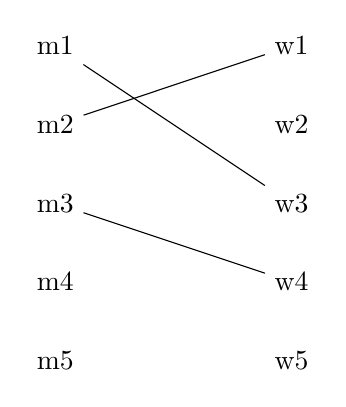
\begin{tikzpicture}[black/.style={circle,draw,fill=black,inner sep=0pt, minimum width=4pt}]
\node at (1,4) (m1) {m1};
\node at (1,3) (m2) {m2};
\node at (1,2) (m3) {m3};
\node at (1,1) (m4) {m4};
\node at (1,0) (m5) {m5};
\node at (4,4) (w1) {w1};
\node at (4,3) (w2) {w2};
\node at (4,2) (w3) {w3};
\node at (4,1) (w4) {w4};
\node at (4,0) (w5) {w5};

\draw (m1) -- (w3);
\draw (m2) -- (w1);
\draw (m3) -- (w4);
\end{tikzpicture}

\end{figure}
Starting at step 1 of the algorithm, we choose $x$ and $y$ as our basic vertices, and name $x=1-2$ and $y=2-3$.
Continuing to step 2, we find two vertices adjacent to both basic vertices: $z$ and $v$.
There are two such vertices, so we continue to step 4.
$z$ and $v$ are not adjacent, so they make two distinct triangles.
The triangle $(x,y,z)$ is odd, so we call $z=2-4$, and $v=1-3$.
We now skip to step 6, and use our fully named $1-clique$ to successively half-name all vertices adjacent to it: $w=3-6$, and $u=1-5$.
Now at step 8, we choose a half-named vertex, $u$.
It is adjacent to a fully named vertex, $x$.
$x$ and $v$ fully name $u$.
We continue this for the remaining vertices, and we obtain the graph below:

\begin{figure}[H]
\centering
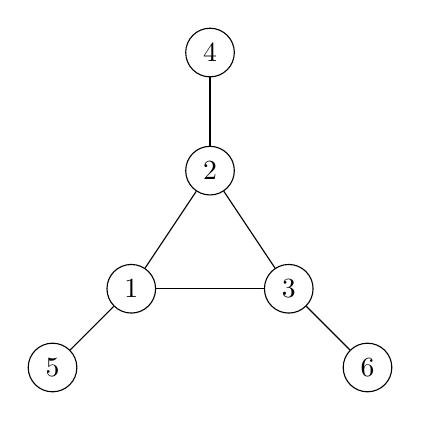
\begin{tikzpicture}[black/.style={circle,draw,fill=black,inner sep=0pt, minimum width=4pt}]
\node[circle,draw] at (1,1) (1) {1};
\node[circle,draw] at (0,0) (5) {5};
\node[circle,draw] at (3,1) (3) {3};
\node[circle,draw] at (2,2.5) (2) {2};
\node[circle,draw] at (2,4) (4) {4};
\node[circle,draw] at (4,0) (6) {6};

\draw (1) -- (2);
\draw (1) -- (3);
\draw (2) -- (3);
\draw (4) -- (2);
\draw (5) -- (1);
\draw (6) -- (3);
\end{tikzpicture}

\end{figure}

It is simple to check that the line graph of the graph below is isomorphic to the original graph, and so the graph we were given was indeed a line graph, and the graph we constructed is its root graph.


\section{Optimization}

\subsection{Find a maximum clique in a line graph}

Given a graph $L(G)$, finding a vertex of degree $\Delta(G)\neq3$ in $G$ corresponds to finding a maximum matching in $L(G)$.
Since this algorithm runs in linear time, if $L(G)$ is indeed the line graph of some simple graph $G$, then we can find a maximum clique -- normally a very computationally hard problem -- efficiently by transforming one from a degree $\Delta(G)$ vertex in $G$.


\subsection{Find a maximum independent set in a line graph}

Given a graph $L(G)$, finding a maximum matching in $G$ corresponds to finding a maximum independent set in $L(G)$.
Since this algorithm runs in linear time, if $L(G)$ is indeed the line graph of some simple graph $G$, then we can find a maximum independent set -- normally a very computationally hard problem -- efficiently by transforming one from a maximum matching in $G$.


\bibliography{p3}
\bibliographystyle{plain}


\end{document}
